\documentclass{article}
\usepackage[utf8]{inputenc}
\usepackage{graphicx}

\title{Secure localisation}
\author{Bastian Fredriksson}
\date{\today}

\begin{document}

\maketitle
\noindent
\verb!Course: Advanced Networked Systems Security, Lecture 4!\\
\verb!Lecturer: Panos Papadimitratos!
\section{Distance-bounding protocols}
Distance-bounding protocols aims to ensure that a prover is within a specific distance. Consider the scenario where an intruder Trudy wants to get access to a building protected by an RFID reader. Trudy positions herself with an RFID tag connected to a long-distance radio. When the reader sends the challenge, it is relayed (forwarded) over radio to Trudys friend Mallory who is in close proximity to Bob with access to the building. Bob has an RFID card in his pocket which responds to the challenge. The response is sent back over radio to Trudy, who forwards the response back to the reader. Since the response is legit (produced by Bob), Trudy will be let into the building. This attack is sometimes called a \textit{relay attack} or \textit{mafia fraud attack}. A possible solution to this problem is to implement a distance-bounding protocol as a part of the authentication process.

An example of a distance-bounding protocol based on a rapid-bit exchange is described in \cite{Brands1994}. In this protocol, the prover $P$ and the verifier $V$ exchange $2k$ bits in such a way that bit $b_{i}$ is sent immediately after bit $b_{i-1}$ is received. $P$ starts by committing to $k$ random bits using a commitment scheme. After the rapid bit exchange, $V$ can determine an upper-bound on the distance to $P$ by computing the maximum response time between each corresponding send and receive operation. Finally $P$ sends a signature of all $2k$ bits to $V$ to prove they were received correctly. This scheme achieves protection against the mafia fraud attack with probability $1-\frac{1}{2^k}$.
\section{Secure localisation}
Distance-bounding protocols are an important building block in secure location protocols where one want to verify 1) The position of other neighbours or 2) Your own position. An example of such a protocol verifying the position of other neighbours is described in \cite{fiore13}. The protocol is depicted in \ref{fig:secureloc}.

The following assumptions are made:
\begin{enumerate}
    \item Each node has an identity consisting of keypair, which can be used to sign, encrypt and decrypt data.
    \item Nodes are working in promiscious mode, e.g they can overhear traffic sent by other nodes.
    \item Node positions do not vary significantly during protocol execution. Relative spatial movements are taken into account using the tolerance value $e_m$.
\end{enumerate}
\noindent
The protocol is executed in four steps as shown in \ref{fig:secureloc}, and consists of four steps. The node $S$ who want to verify the location of other nodes starts by broadcasting a POLL packet containing a temporary public key $K'_s$. Any node receiving such a packet broadcasts REPLY packet containing a challenge $C_x$ with a nonce $p_x$ and the reception time, encrypted using the public key $K'_S$, together with the hash of the public key.

The reception time $t_{YX}$ of any reply packet is stored by each of the neighbours. When $S$ sends a REVEAL packet (revealing his identity using his real MAC address), each of the neighbours responds with a unicast to $S$ containing its position $GPS_X$, the transmission time of his reply packet, and a map, mapping an identifier $i_z$ for node $Z$ (as specified in $S$ REVEAL packet) to a time $t_{YX}$, specifying the time when $X$ received $Z$:s REPLY packet.
\begin{figure}
    \centering
    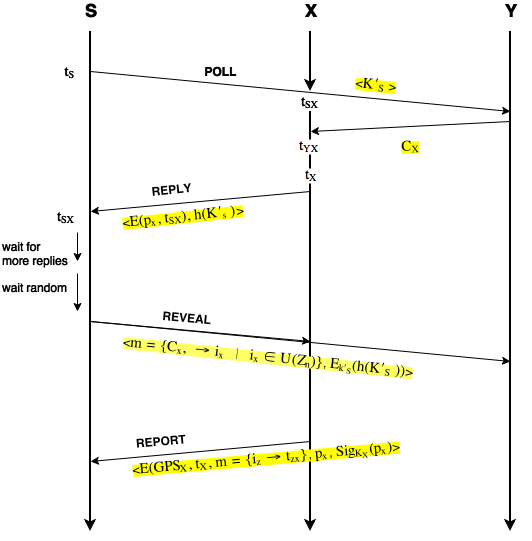
\includegraphics[width=12cm]{secureloc}
    \caption{The protocol used to exchange location information. Note that the POLL packet is completely anonymous. It is sent from a spoofed MAC and contains a temporary public key $K'_s$. Any adversary overhearing the traffic cannot know the identity of the node requesting the information until a REVEAL packet is sent.}
    \label{fig:secureloc}
\end{figure}

After the protocol execution, $S$ can use the timings to compute the time of flight (ToF) for each each packet, deriving the approximate distance to each of the neighbours. $S$ then runs three tests to categorise the neighbours into three different categories 1) Verified - with nodes who appears to have answered with a correct location 2) Faulty - with nodes who appears to have answered with a fake location and 3) Unverified - with nodes where we are unable to determine the truthfulness of the reply.
\noindent
The tests are as follows:

\begin{enumerate}
    \item \textbf{The direct symmetry test (DST)} - For every neighbour $X$, checks whether the distance between $X$ and $S$ is equal to the distance between $S$ and $X$. Secondly, makes sure that the time of flight between $S$ and $X$ corresponds to the advertised distance between their positions. Thirdly, that they are not farther away than $R$ the maximum communication distance. If so, mark $X$ as faulty.
    \item \textbf{Cross-symmetry test (CST)} - For every pair $(X, Y)$ of neighbours, who are not collinear with $S$ or marked as faulty by DST, increment a link counter and perform the same checks as in DST but between $X$ and $Y$ instead of between $S$ and $X$. If one of the checks fails, a mismatch counter is incremented. After each pair of neighbours has been checked, a node is marked as faulty iff the ratio between the mismatch counter and the link counter exceeds some specified value $0 \le \delta \le 1$. Otherwise, mark a node as verified, if it has at least two neighbours (link counter is at least 2).
    \item \textbf{The multilateration test (MLT)} - Looks for suspect neighbours marked as verified by CST. A neighbour $X$ is considered suspect if it says that it can reach another neighbour $Y$ (has received a reply packet from $Y$), but not the other way around. For every such pair $(X, Y)$, create a hyperbola for $X$, which represents the set of possible positions for $X$. In the end, we can multilaterate the position of $X$ using the intersection between two or more hyperbolas. $X$ is marked as faulty if the multilaterated position differs (by a significant amount) from the position advertised by $X$.
\end{enumerate}
\noindent
The scheme is shown to be secure against a wide range of different attacks. However, it would be possible to break the scheme if the majority of nodes are adversarial for $\delta = 0.5$. In this case, they can cooperate to multilaterate the position of $S$ and advertise (consistent) fake timings which supports their (fake) position.
\bibliographystyle{acm}
\bibliography{ref}
\end{document}
